\section{Vector spaces and fields}\label{real-and-complex-vector-spaces}
A vector in a vector space is just something which can be added to another vector from the vector
space, and scaled by a scalar from the associated field. A vector does not involve any numbers until
it is represented as a linear combination of basis vectors, using scalars from the associated
field. So whether something is a ``real vector space'' or a ``complex vector space'' depends only on
the field. If the field is $\R$ it is a real vector space; if the field is $\C$ it's a complex
vector space. It doesn't make sense to ask whether the vectors themselves are real or complex.

A \defn{field} is a set which is an abelian group under both addition and multiplication.

A \defn{vector space} is an additive abelian group $X$, together with a field $F$, such that $X$ is
closed under linear combinations with scalars from the field $F$.

\subsubsection{Examples}

TODO:
\begin{itemize}
\item clarify: is $\C$ a field or a vector space or both?
\item What is a one-dimensional complex vector space?
\end{itemize}

\begin{enumerate}
\item $\R$ is a field.

\item $\R^2$ is not a field; multiplication is undefined.

\item If we equip $\R^2$ with complex multiplication then this is the field called $\C$.

\item The additive abelian group $\R$, together with the field $\R$, is a one-dimensional vector space.

  {\bf Proof:} Let $x \in \R$ with $x \neq 0$. Then $\{x\}$ is a basis for $\R$, since every element of $\R$ can
  be expressed uniquely as a scalar multiple of $x$. So $\R$ is one-dimensional.

\item The additive abelian group $\R^n$, together with the field $\R$, is a vector space. It is $n$-dimensional.

\item The additive abelian group $\C$, together with the field $\R$, is a two-dimensional vector
  space. It is isomorphic to $\R^2$.

\item The additive abelian group $\C$, together with the field $\C$, is a one-dimensional vector space.

  {\bf Proof:} Let $z \in \C$ with $z \neq 0$. Then $\{z\}$ is a basis for $\C$, therefore $\C$ as a
  complex vector space is one-dimensional.

\end{enumerate}

\newpage
\section{The qubit}
The state of a qubit is a unit vector in a two-dimensional complex vector space. The basis vectors
are written $\ket{0}$ and $\ket{1}$, so a qubit is
\begin{align*}
\alpha\ket{0} + \beta\ket{1}
\end{align*}
where $\alpha, \beta \in \C$ with $|\alpha|^2 + |\beta|^2 = 1$.

What does the normalization constraint $|\alpha|^2 + |\beta|^2 = 1$ mean geometrically? If
$\alpha = 0$ then $\beta$ lies on the unit circle, and vice versa.

How can we visualize the possible values of a qubit? How about this: visualize $(|\alpha|, |\beta|)$
as a point on the unit circle and place a clockface at that point with two hands, representing the argument
of $\alpha$ and $\beta$.\\
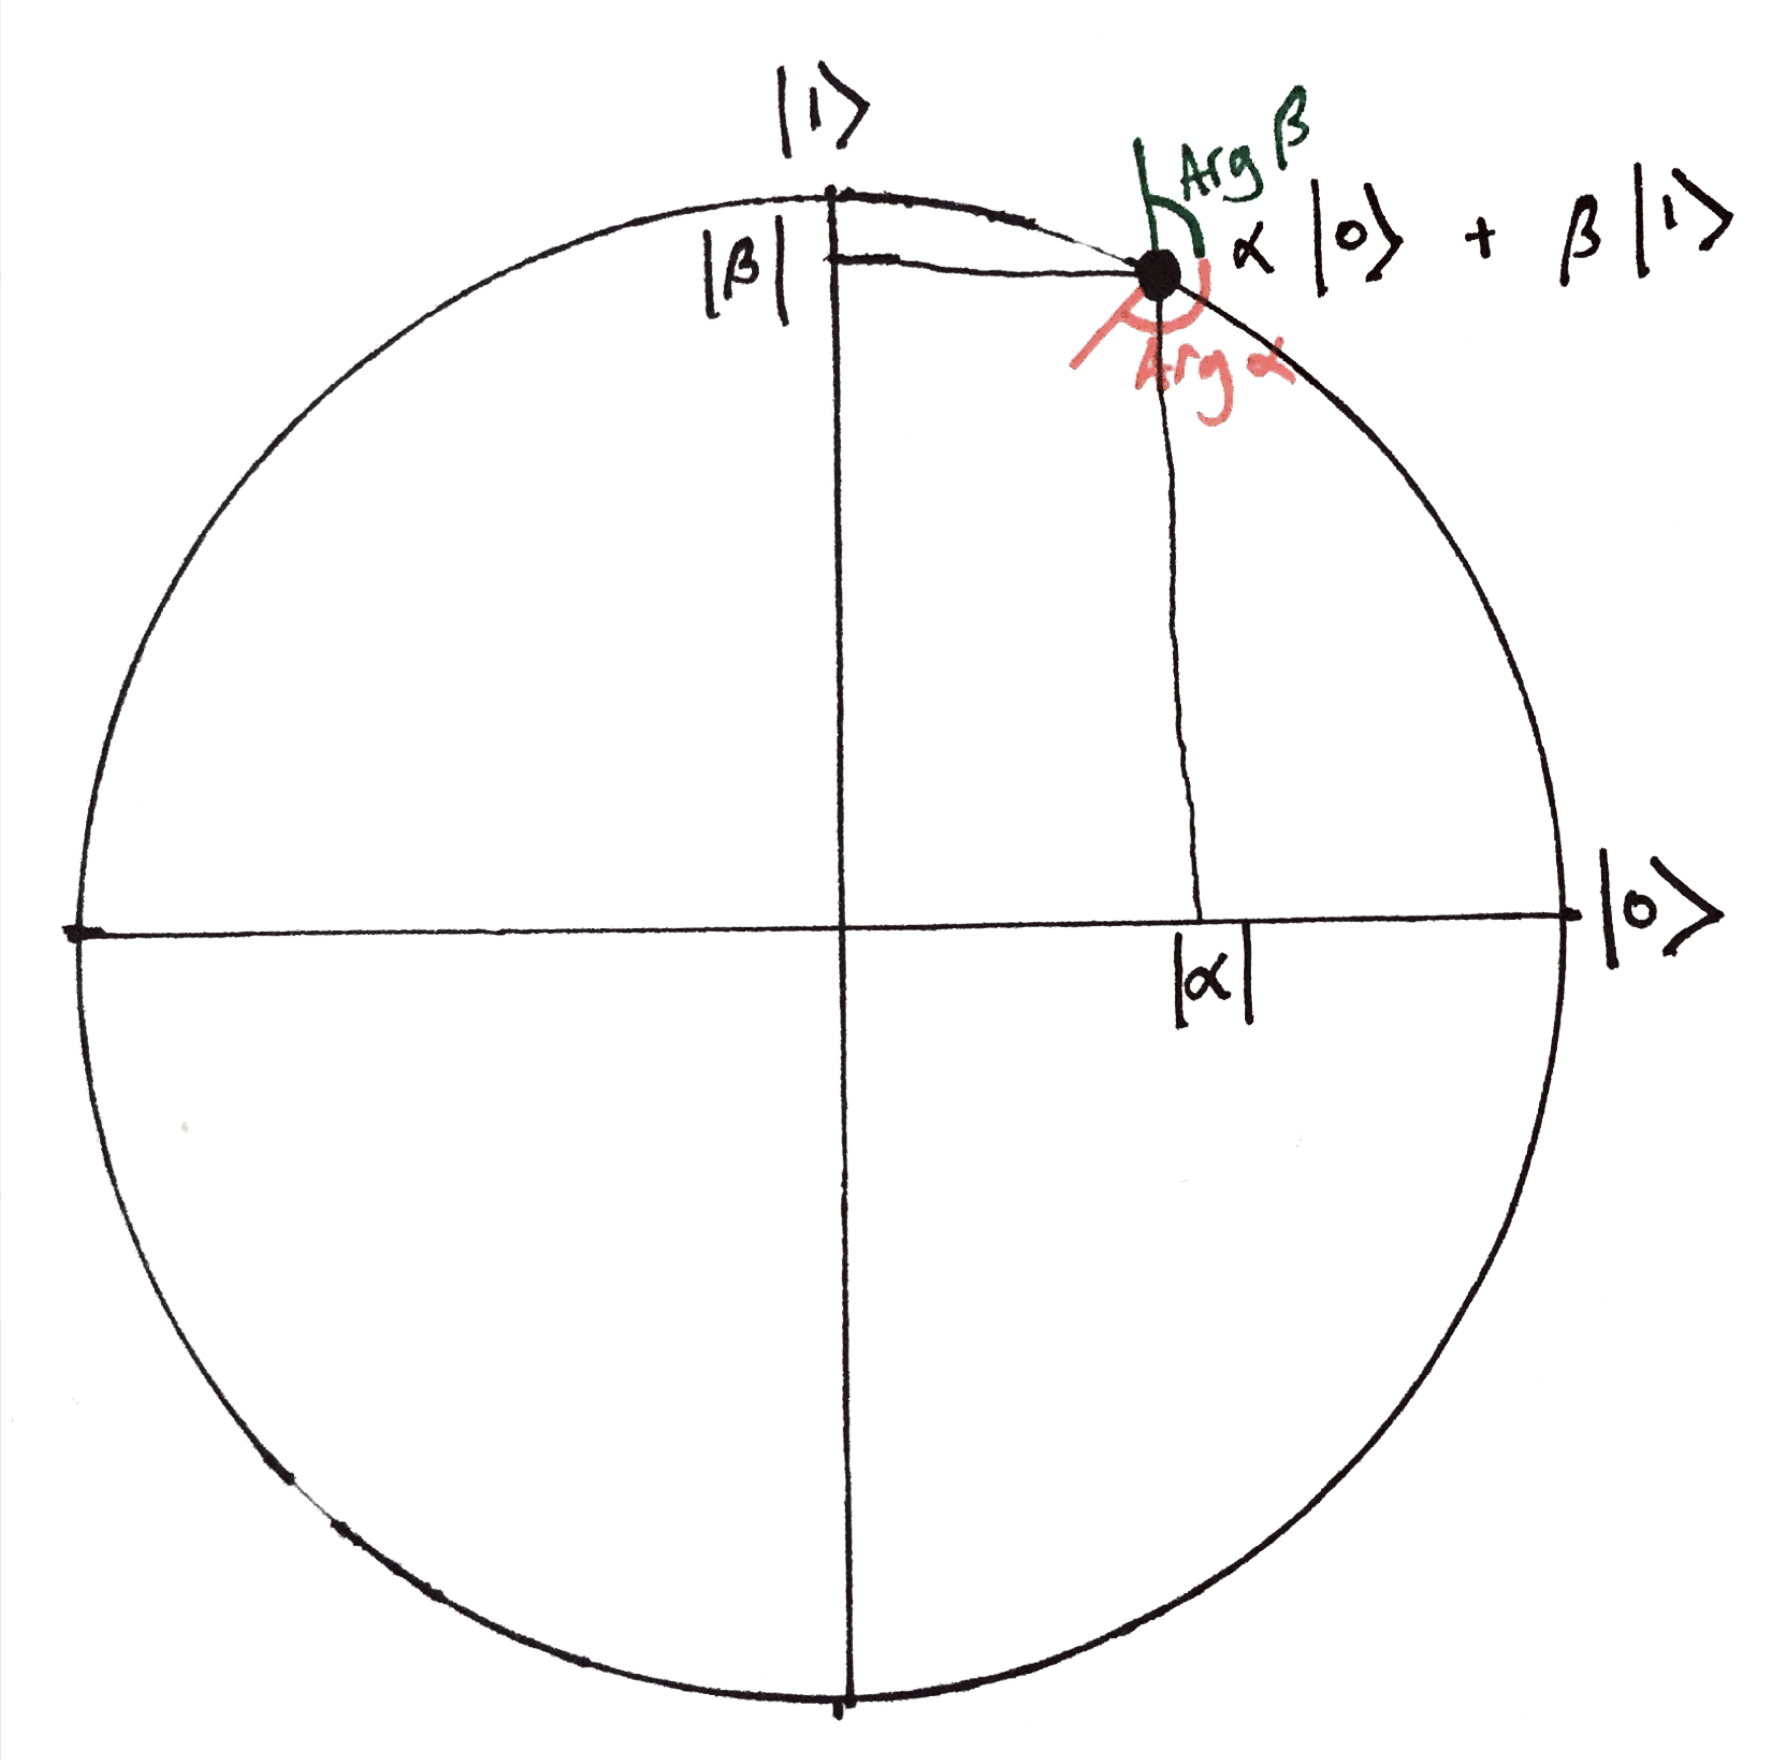
\includegraphics[width=200pt]{img/quantum-qubit.png}


\section{Quantum logic gates}
\subsection{NOT}
\begin{align*}
  \ket{0} &\mapsto \ket{1}\\
  \ket{1} &\mapsto \ket{0},
\end{align*}
so by linearity
\begin{align*}
  \alpha \ket{0} + \beta \ket{1} \mapsto \alpha \ket{1} + \beta \ket{0}.
\end{align*}
Matrix representation:
\begin{align*}
  \matMMxNN{0}{1}
           {1}{0}
\end{align*}